
\chapter{Referencial Teórico e Trabalhos Relacionados}
\label{cap:referencial-teorico}

  A seguir nós discutimos conceitos e trabalhos relacionados sobre a visualização de
trajetórias com foco em dados de Origem-Destino. Apresentamos inicialmente as propriedades
desse tipo de dado juntamente com uma taxonomia que os divide conforme os diferentes cenários para
sua visualização e exploração. Em seguida, destacamos o \emph{bundling},
uma técnica bastante usada na visualização de grandes quantidades de dados de trajetórias.

\section{Visualização de Trajetórias}
\label{sec:dados-de-trajetorias}

Dados de \emph{trajetórias} (aqui também nomeadas como fluxos ou tráfego)
formam conjuntos de pontos no espaço $\mathbf{t} = \{\mathbf{x}_i\}$, que quando
capturados em momentos consecutivos $t_i$ descrevem o movimento de um objeto ao
longo do tempo. Uma trajetória pode conter outras informações, capturadas em
cada passo $\mathbf{x_i}$, \emph{e.g.}, velocidade, ou ainda atributos globais
que permeiam todos os instantes, \emph{e.g.}, tipo de veículo.

A análise e visualização desse tipo de dado tem um histórico antigo, e para
compreender melhor os esforços nesse campo de estudo, um levantamento feito por
\citet{Chen2015} traz uma caracterização sobre várias pesquisas de visualização
de dados de trajetórias existentes, que incluem tráfego de pessoas, carros,
embarcações, e outros. Eles apresentam uma taxonomia conforme algumas
características observadas, como o objetivo da visualização, formato dos dados
do tráfego e formas de apresentação de suas propriedades. Nesta seção
apresentamos essa taxonomia, que é importante para um melhor entendimento da
área.

\subsection{Quanto ao Tipo de Coleta de Dados}

Dados de trajetórias são tipicamente coletados a partir de sensores e
dispositivos eletrônicos e sua estrutura depende do modo de operação desses
equipamentos que registram a movimentação dos objetos. \citet{Chen2015} os dividem em três classes:

\begin{itemize}
  \item \textbf{Baseado em pontos de interesse:} a posição de um objeto é
gravada assim que ele entra na área do sensor. Como uma câmera de vídeo que
capta a movimentação e orientação de um veículo assim que ele passa pela área de
monitoramento.

  \item \textbf{Baseado em ações:} as informações sobre um objeto podem estar
associadas a certas atividades. O usuário de um aparelho celular por exemplo,
tem sua atividade e localização registradas pela rede da operadora
quando o mesmo efetua uma chamada.

\item \textbf{Baseado em sinais de dispositivos:} um dispositivo de localização,
como aparelhos de GPS, grava e envia a trajetória de um objeto para uma central
\end{itemize}

A frequência de armazenamento dessas informações também impacta a análise.
Capturar e armazenar essas informações com um intervalo de tempo muito pequeno
pode ser algo bastante custoso, por isso, algumas aplicações acabam por
armazenar apenas a Origem e o Destino (OD). Outro fator de impacto é a precisão
das informações a qual depende de questões relacionadas ao hardware utilizado na
coleta. Muitas vezes é necessária uma etapa de pré-processamento para extrair
dados inconsistentes da análise.

\subsection{Quanto ao Objetivo da Visualização}

Ainda segundo \citet{Chen2015}, os trabalhos levantados sobre visualização e análise
de dados do tráfego podem ser classifcados em quatro categorias de
acordo com seus objetivos e a tarefa a que servem.

\begin{itemize}
  \item \textbf{Monitoramento do tráfego:} esse tipo de análise foca no
monitoramento em tempo real para descobertas instantâneas de eventos no tráfego,
como câmeras de gravação ao vivo e sistemas de alerta.

  \item \textbf{Descoberta de padrões e clusterização:} para a descoberta de
padrões e tendências de mobilidade, algumas aplicações utilizam algoritmos
de clusterização para agrupar visualmente as trajetórias e destacar
o comportamento de certos grupos, geralmente utilizando dados históricos
do tráfego.

  \item \textbf{Exploração e predição:} outras análises focam em fornecer
mecanismos de pesquisa e exploração dos dados para que os usuários investiguem
situações do tráfego, como descobrir a causa de um congestionamento no trânsito,
ou ainda técnicas de predição para prever essas situações (e.g. predizer que
haverá congestionamento devido a ocorrência de chuva).

  \item \textbf{Planejamento de rotas e recomendação:} nessa categoria, 
os dados do tráfego são usados essencialmente para criar recomendações de trajetos para usuários
do transporte. Várias soluções existem com esse propósito, que podem envolver
monitoramento em tempo real ou análise histórica no processo de recomendação.
\end{itemize}

\subsection{Visualização das Propriedades Temporais}

Dados do tráfego podem conter uma série de variáveis, das quais as mais
importantes são o tempo e espaço. Visualizações orientadas ao tempo enfatizam
tendências, periodicidades e anomalias nos dados ao longo de um eixo que destaca
essas propriedades temporais \citep{Aigner2008}. Expressar a variação do tráfego
ao longo do tempo e sua evolução é um típico processo de análise linear do
tempo que considera a informação desde um ponto de início até um ponto final
\citep{Chen2015}. 

Uma maneira comum de projeções que enfatizam as informações temporais
são gráficos de linhas, onde o tempo é colocado ao longo do eixo X e outra variável
é representada no eixo Y, como mostra a Figura \ref{fig:linear-time}. Esse tipo
de visualização é fácil de representar, porém limitam-se na quantidade de
variáveis que podem ser visualizadas.

\begin{figure}[!htb]
  \centering
  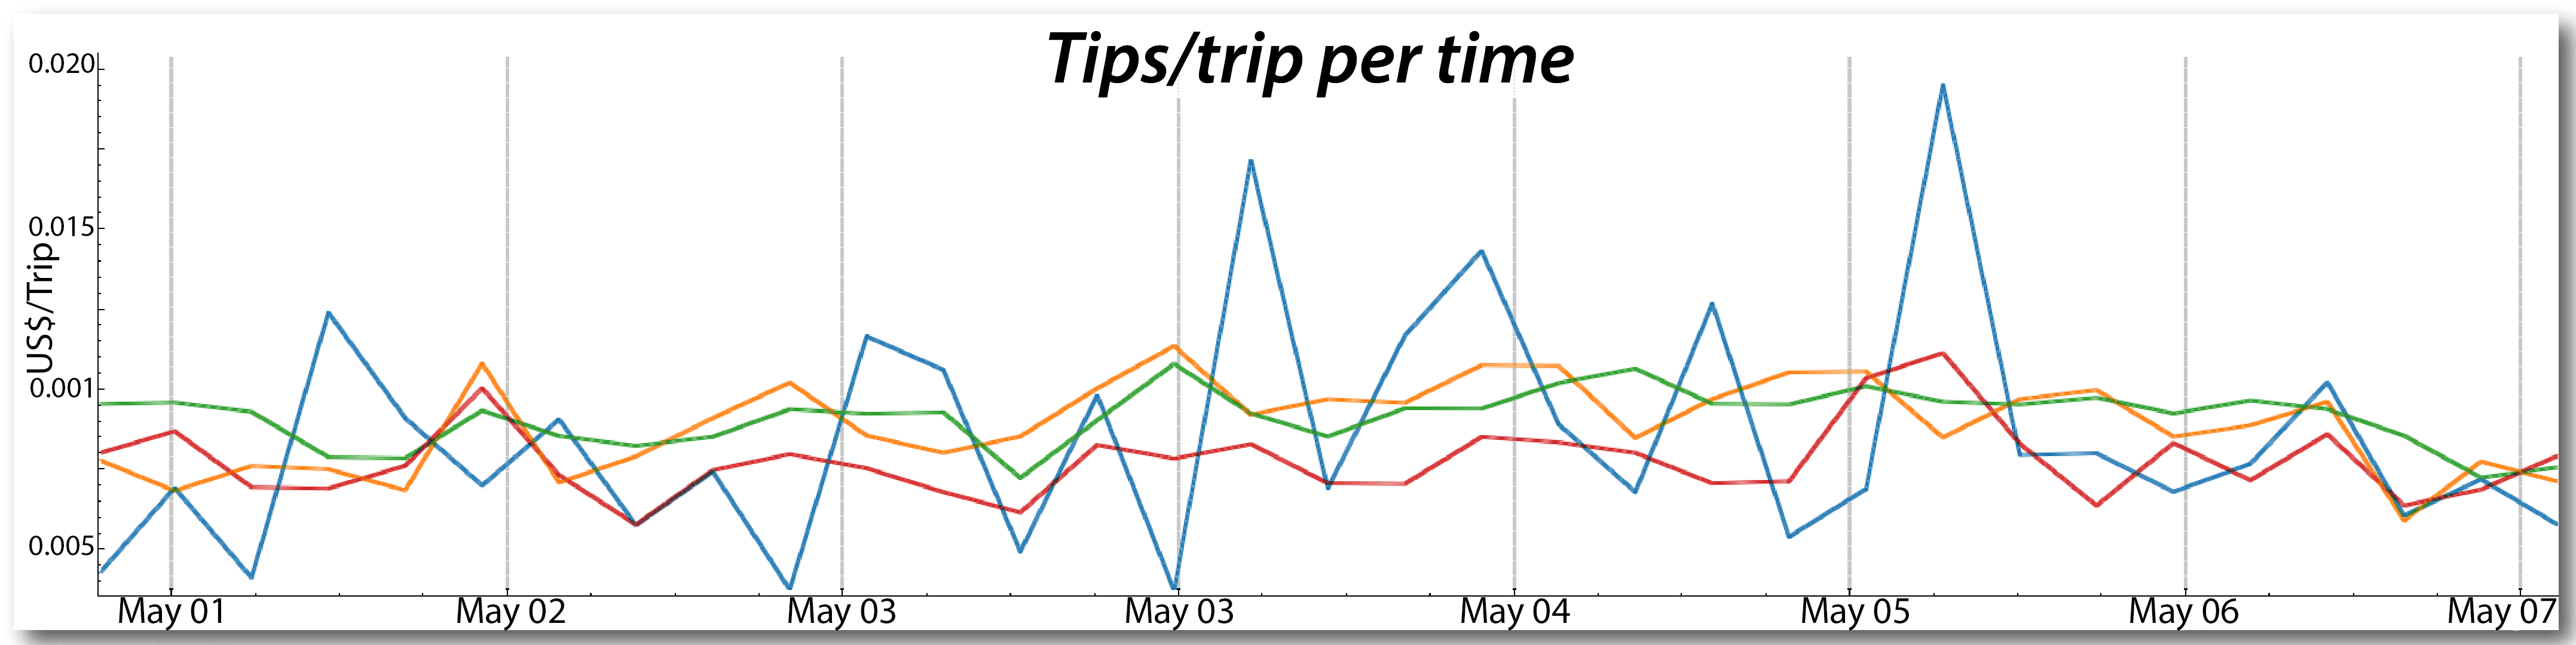
\includegraphics[width=\textwidth]{../figuras/linear-time.png}
  \caption[Gráfico de linha representando tempo linear]{Gráfico de linha representando tempo linear. 
Ele mostra o valor médio de gorjetas em viagens de taxi em 4 regiões de Nova Iorque no período de 1 a 7 de Maio de 2011.
Cada linha representa uma região. Fonte: \citep{Ferreira2013}
  \label{fig:linear-time}}
\end{figure}

Por outro lado, temos também alguns processos recorrentes que são naturais em nosso
mundo, os quais seguem ciclos de estações, ou mesmo ciclos semanais e diários. Um leiaute
radial visto na Figura \ref{fig:periodic-time} é uma opção para se visualizar essa periodicidade. O tempo é
mostrado no eixo circular e cada anel do círculo representa um dia da semana. Os setores
representam uma hora, com 24 setores no total que mostram a quantidade de tráfego em
um determinado ponto da cidade, mapeada em cores. A vantagem de um leiaute radial
é que ele evidencia esses padrões recorrentes e a desvantagem é que ele possui pouca
eficiência espacial, \citep{Chen2015}.

\begin{figure}[!htb]
  \centering
  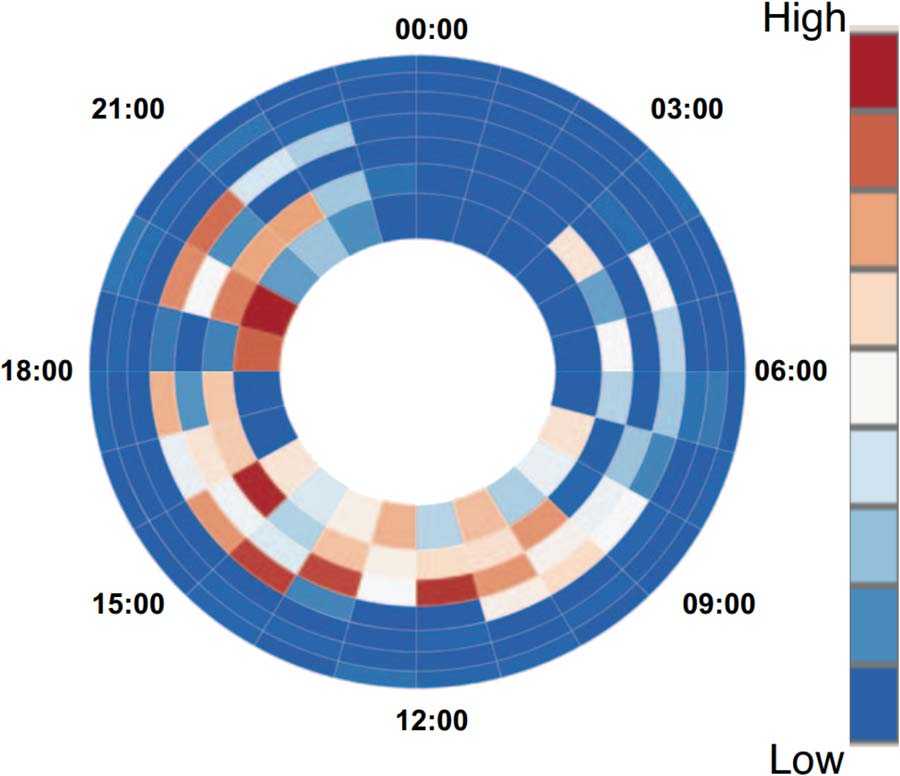
\includegraphics[width=0.6\textwidth]{../figuras/periodic-time.png}
  \caption[Leiaute radial representando tempo periódico]{Leiaute radial
representando tempo periódico. O tempo é mostrado no eixo circular e cada anel
do círculo representa um dia da semana, divididos em 24 setores que indicam as
24 horas do dia. As cores mostram a quantidade de tráfego conforme o mapa à
direita, onde vermelho maior é o tráfego. Fonte:
\citet{Pu2013} \label{fig:periodic-time}}
\end{figure}


% Dados de trajetórias podem ser diretamente desenhados sobre mapas 2D,
% e outros atributos representados através de elementos visuais como cor e textura.
% As propriedades espaciais de localização, que referem-se
% aos locais onde ações, incidentes e eventos ocorreram, é a principal característica
% desse tipo de dado e pode ser agregada de diferentes formas, as quais \citet{Chen2015}
% separa em três categorias: \emph{visualização baseada  em pontos} (nenhuma agregação), \emph{visualização baseada em linhas}
% (agregação de primeira ordem), e \emph{agregação baseada em regiões} (agregação de segunda ordem).




Visualizações baseada em pontos (nenhuma agregação)
consideram as informações do tráfego como pontos discretos e usam sua forma
pura como representação em um leiaute espacial, como pontos individuais em um mapa 2D.
Essa tipo de visualização mostra a posição instantânea dos objetos em um certo momento
no tempo. A vantagem desse método é que ele mostra um retrato dos estados de cada objeto em um
determinado momento, permitindo observar sua distribuição no espaço e explorar regiões que estejam
mais ocupadas. Para entender mudanças contínuas ao longo do tempo, técnicas de animação podem
ser empregadas para mostrar uma transição entre os estados. Porém, com um grande número de partículas
- alguns milhares de pontos - esse tipo de visualização começa a sofrer
de um efeito conhecido como como movimento Browniano - onde o movimento dos pontos parecem ser movimentos
aleatórios - o que torna difícil identificar a trajetória dos objetos. O projeto \emph{Trains of Data},
ilustrado na Figura \ref{fig:trains-of-data}, utiliza esse tipo de visualização para
representar a movimentação dos trens na França. O tamanho dos pontos indica a quantidade de passageiros e a cor
sua assiduidade, verde se o trem está no horário e vermelho significa que está atrasado
em relação ao tempo estimado.

\begin{figure}[!htb]
  \centering
  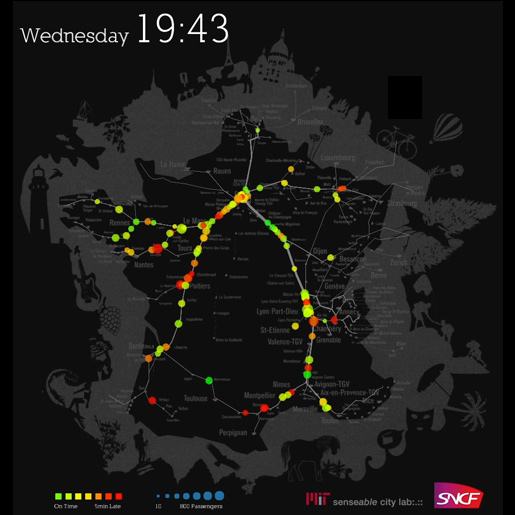
\includegraphics[width=.6\textwidth]{../figuras/trains-of-data.jpg}
  \caption[Visualização baseada no mapa das ferrovias da França]{Posição dos trens às 19:43 na França com uma visualização baseada no mapa
das ferrovias. Fonte: \citet{Senseable2018}.}
  \label{fig:trains-of-data}
\end{figure}

Visualizações baseadas em linhas (agregação de primeira ordem) são
desenhadas para mostrar a trajetória de objetos, mapas de vias e estradas em
uma região, ou fluxos do tráfego em uma rede de transporte. As trajetórias e
fluxos são representados por linhas ou curvas e são escaladas ou coloridas de
acordo com suas propriedades (i.e. densidade, direção, velocidade) e mostram de forma
explicita a conexão entre diferentes localidades espaciais. \citet{Klein2014} apresenta
um sistema iterativo para análise do tráfego aéreo na França. As trajetórias são
representada por linhas que conectam os pontos de partida e chegada de cada voo,
como pode ser visto na Figura \ref{fig:air-traffic}.

\begin{figure}[!htb]
  \centering
  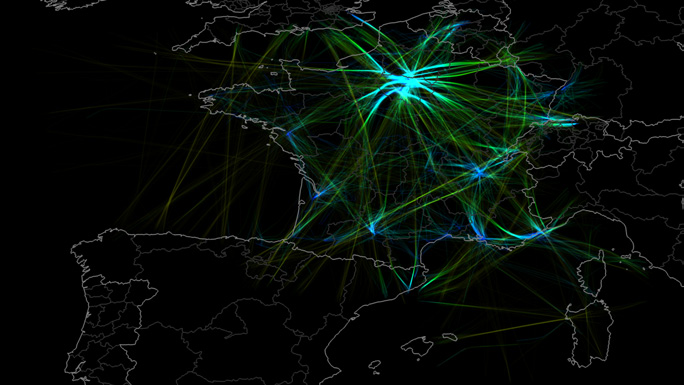
\includegraphics[width=1\textwidth]{../figuras/air-traffic.png}
  \caption[Visualização do tráfego aéreo na França]{Visualização do tráfego aéreo na França. Fonte: \citet{Klein2014}.}
  \label{fig:air-traffic}
\end{figure}

A representação espacial das linhas pode ainda sofrer transformações
geométricas e topológicas que geram novas abstrações. Por exemplo,
\citet{Tarik2009} mostram uma proposta que transforma as trajetórias de um
leiaute espacial (Figura \ref{fig:viz-espacial}) para um leiaute abstrato
(Figura \ref{fig:viz-abstrata}) para visualizar a movimentação de pessoas
durante a fuga de uma explosão em um escritório. A abordagem abstrata é usada
para mostrar mais efetivamente os padrões de movimentação de pessoas que se
movem ao mesmo tempo para as mesmas áreas. Na Figura \ref{fig:viz-abstrata} é
possível notar a movimentação de indivíduos antes da explosão (linhas azuis), o
que sugere possíveis suspeitos ou testemunhas do evento.  As informações
temporais são difíceis de representar no leiaute espacial, assim o leiaute
abstrato complementa a visualização dos dados mostrando os instantes de tempo
no eixo X e as informações espaciais no eixo Y.

\begin{figure}[ht!]
  \centering
  \begin{subfigure}[t]{0.45\textwidth}
    \centering
    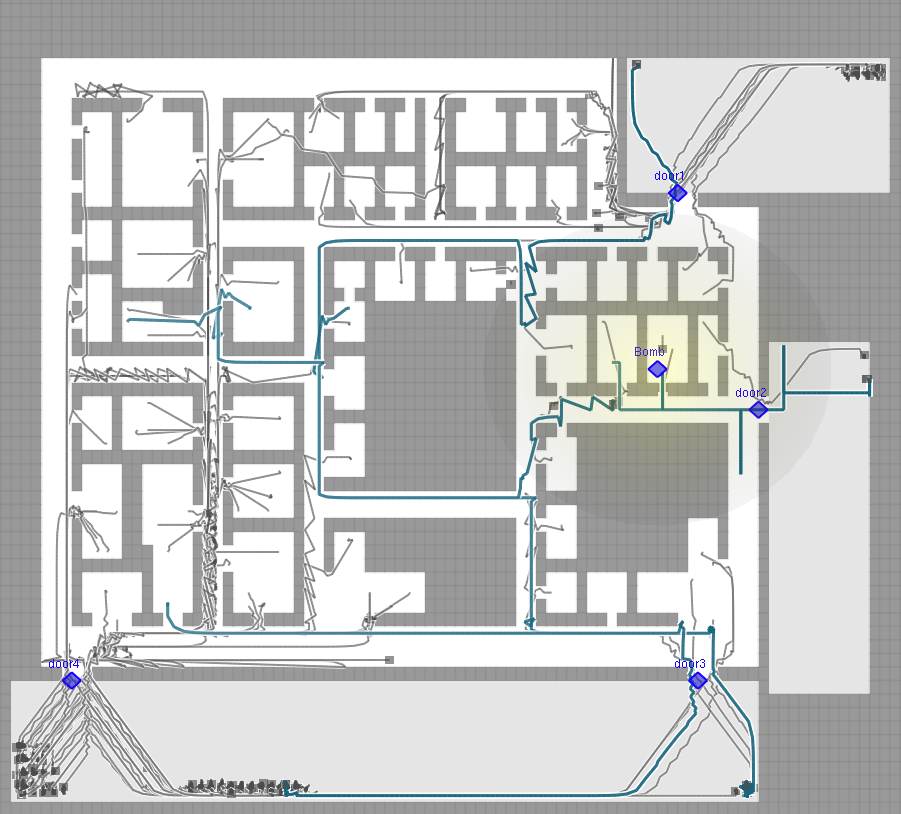
\includegraphics[width=65mm]{../figuras/proximidade-espacial.png}
    \caption{Visualização espacial das trajetórias ao longo do tempo. \label{fig:viz-espacial}}
  \end{subfigure}
  ~
  \begin{subfigure}[t]{0.45\textwidth}
    \centering
    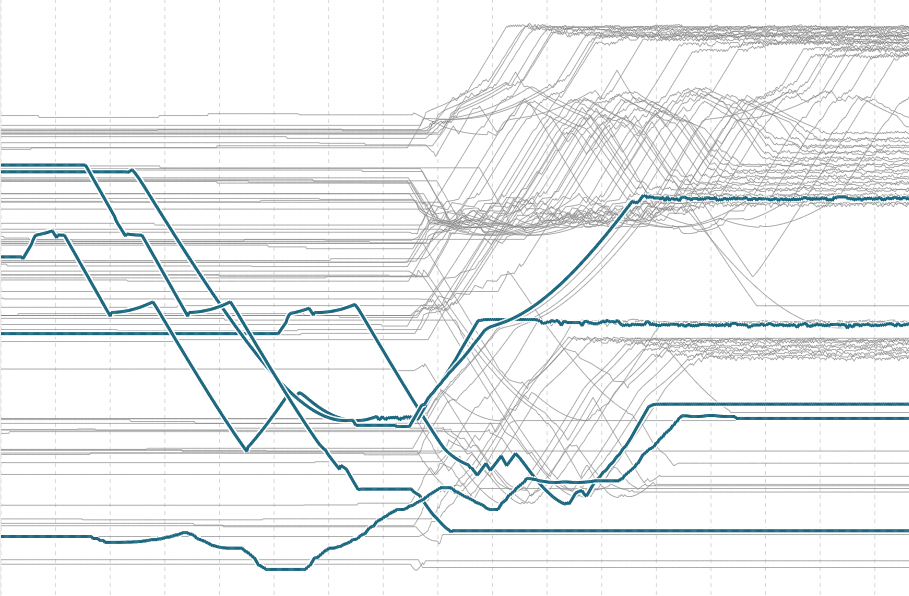
\includegraphics[width=75mm]{../figuras/proximidade-abstrata.png}
    \caption{Visualização abstrata da movimentação ao longo do tempo. \label{fig:viz-abstrata}}
  \end{subfigure}

  \caption[Visualização espacial vs abstrata da movimentação de pessoas]{Simulação de uma evacuação de um escritório depois de uma explosão.
(a) Visualização da movimentação da trajetória das pessoas no espaço. (b)
Visualização abstrata, baseada na proximidade.  Fonte: \citet{Tarik2009}.
\label{fig:tarik}}
\end{figure}

No entanto, a medida que o número de linhas cresce, aumenta também os
problemas de oclusão, o que acaba afetando a estética da visualização e a
obtenção de informações sobre os dados \citep{Zhou2013}. Visualizações baseadas
em regiões (agregação de segunda ordem) são uma forma de reduzir
a complexidade de análise de um grande conjunto trajetórias. Os dados 
são então agrupados em um nível de macro regiões, geralmente determinado por divisões administrativas.
\citet{Zeng2013} apresentam um diagrama em círculos para mostrar padrões de movimentação de
pessoas entre as regiões da cidade. O círculo representa a junção ou conexão
entre as diferentes regiões e o fluxo entre elas. A densidade do fluxo é medido
pela espessura, bem como a direção é destacada dentro do círculo, como é
ilustrado na Figura \ref{fig:interchange-circo}. Esse tipo de agrupamento
troca as informações individuais de cada trajetória  (como na representação de linhas e pontos)
em favor de uma visão condensada, tornando possível a exploração de maiores quantidades de dados, porém
sob uma macro visão da informação.

\begin{figure}[!h]
  \centering
  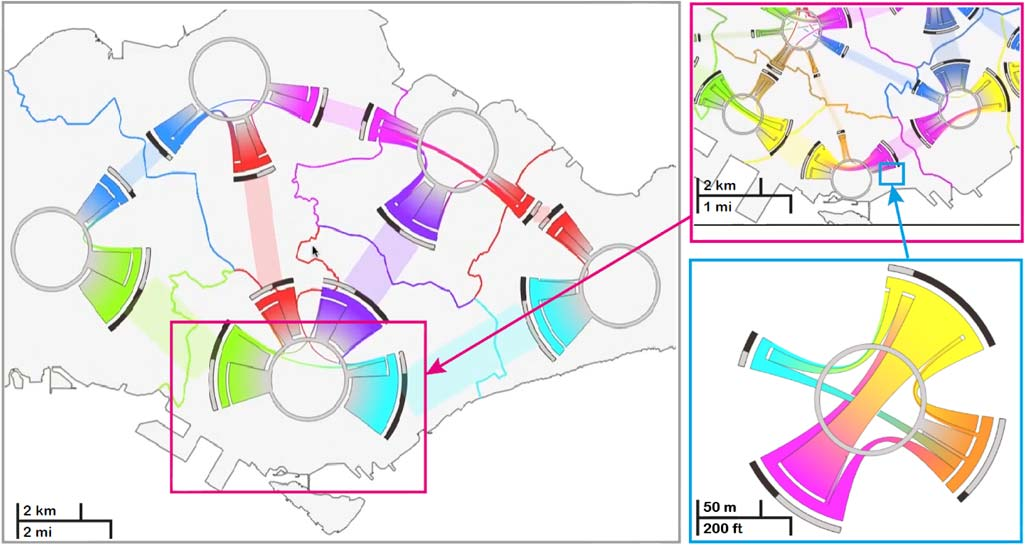
\includegraphics[width=0.97\textwidth]{../figuras/region-based.png}
  \caption[Exemplo de visualização baseada em regiões do sistema de metrô na França]{Exemplo de visualização baseada em regiões: padrões regionais de movimentação no sistema de metrô na França. Fonte: \citet{Zeng2013}.}
  \label{fig:interchange-circo}
\end{figure}

Visualizar conjuntos de trajetórias com dezenas de milhares de fluxos ou mais é um grande desafio.
Desenhar todas as trajetórias em uma imagem resultaria em uma oclusão significativa na visualização,
dificultando a identificação até mesmo dos padrões mais simples que se possa imaginar. Além disso,
há também o desafio de representar os múltiplos atributos, muito comuns nesse tipo de conjunto de dados,
tais como velocidade, direção, tipo de veículo, posição. 

Uma maneira de contornar os problemas de oclusão é através de filtros que determinam
a quantidade de itens na visualização. Porém, como consequência do filtro, perde-se a visão
global de todos os itens ao mesmo tempo, o que pode ser necessário para a identificação das
correlações e padrões entre eles. Uma outra técnica conhecida como \emph{bundling} busca resolver
tais problemas de escalabilidade visual, trazendo um outro tipo de abstração que permite
criar visualizações baseadas em linhas com um grande número de elementos de uma forma simplificada,
que destaca grupos de trajetórias espacialmente próximas, e opcionalmente, que possuam atributos similares.

O \emph{bundling} têm sido utilizado em várias pesquisas sobre dados de movimentação.
\citep{Anita2017} criou uma visualização com \emph{bundling} para estudar características da migração de aves.
\citep{Klein2014} desenvolveu uma visualização dinâmica para mostrar variações do tráfego aéreo ao longo do tempo e
\citep{Willems2009} fez uma análise da movimentação de embarcações marítimas também explorando
técnicas de \emph{bundling}. Separadamente, \citep{Blascheck2017} mostra como a técnica foi
empregada para simplificar a visualização de dados de monitoramento da visão para inferir padrões de leitura. 
Na seção a seguir explicamos como o \emph{bundling} pode ser aplicado para simplificar a exploração
de grandes conjuntos de dados de trajetórias, similares aos dados de OD de nossa pesquisa.

\section{\emph{Bundling}}
\label{sec:bundling}

O conceito geral desta técnica é que os dados das trajetórias são agrupadas em
conjuntos chamados \emph{bundles}. Os \emph{bundles} são definidos como um grupo
de trajetórias similares, compatíveis o suficiente para serem representadas por
um corpo único e compacto \citep{Lhuillier2017}. A compatibilidade é calculada a
partir de uma função de similaridade usada para determinar quais objetos devem
fazem parte do mesmo agrupamento. Imaginando então algumas viagens no trânsito,
é possível agrupá-las pela sua região de origem, destino, distância percorrida,
direção ou o meio de transporte utilizado. A informação agrupada em
\emph{bundles} é ligeiramente inferior ao número de trajetórias a serem
desenhadas, ficando mais simples compreender e visualizar a estrutura global,
padrões e tendências entre grupos de trajetórias que ligam áreas fortemente
relacionadas \citep{Zhou2013}. A Figura \ref{fig:bundling-ex} exemplifica o uso
da técnica de \emph{bundling} em uma visualização baseada em linhas. Os dados
com características similares são agrupados, destacando uma estrutura compacta
que mostra as ligações mais fortes entre as regiões do círculo, sendo que,
quanto mais a direita, maior o nível de agregação dos dados.

\begin{figure}[!htb]
  \centering
  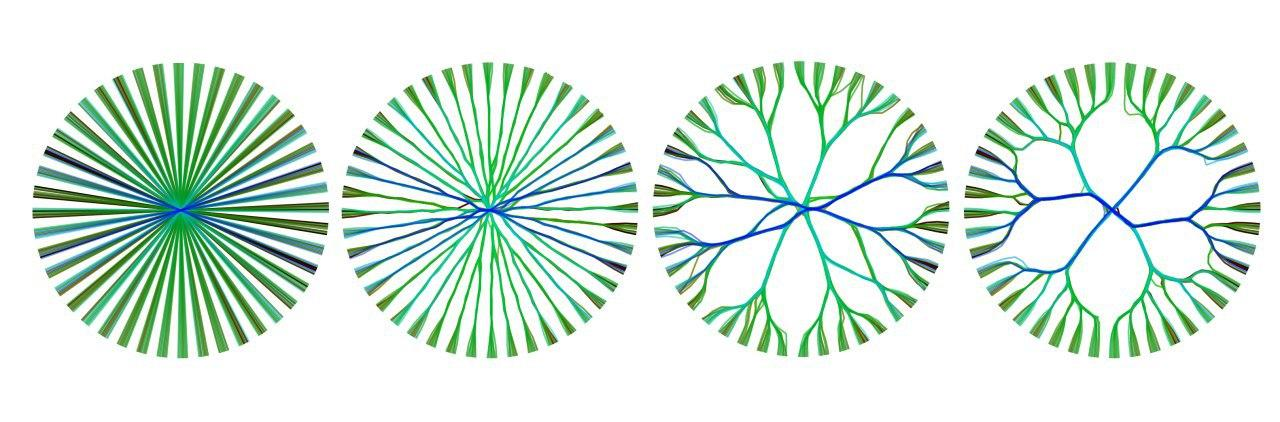
\includegraphics[width=1\textwidth]{../figuras/bundling.jpeg}
  \caption[Exemplo de uma operação de \emph{bundling} aplicado em uma visualização baseada em linhas]{
  Exemplo de uma operação de \emph{bundling} aplicado em uma visualização baseada em linhas. Grupos similares
  são agrupados para desvendar uma macro estrutura dos dados.}
  \label{fig:bundling-ex}
\end{figure}

O cálculo de um \emph{bundle} não possui uma definição precisa, e por isso há
uma grande variedade de algoritmos e abordagens para modelar problemas de
agrupamento de arestas com \emph{bundling}, que podem variar significativamente
de um para outro em questões de complexidade e aplicação dos algoritmos.
\citet{Lhuillier2017} fizeram um estudo sobre o estado da arte das técnicas de
\emph{bundling} e suas aplicações para a análise de dados de trajetórias (como
nossos dados de OD) e dados representados por grafos, mostrando os melhores
métodos para âmbos os casos. Deste estudo, uma classe de algoritmos em particular
se destaca por oferecer vários parâmetros para um maior controle do processo de \emph{bundling}
e também por ser computacionalmente mais eficiente em relação a outros métodos. Conhecidos
como \emph{modelos baseados em imagem}, esses algoritmos são, pelo que conhecemos,
o que há de mais recente no campo de visualização com \emph{bundling}.

\subsection{\emph{Bundling} Baseado em Imagem}
\label{sec:modelo-imagem}

Modelos de \emph{bundling} baseados em imagem (ou \emph{image based bundling
(IBB)}) explorarm, em sua essência, o algoritmo de clusterização \emph{mean
shift} \citep{comaniciu02}, bem conhecido na área de processamento de imagem.
Nós mostramos este processo para uma técnica em particular conhecida como
\emph{Kernel Density Estimation Edge Bundling (KDEEB)}, \citep{hurter:12},
reconhecendo que outras técnicas baseadas em imagem presentes na literatura
funcionam de maneira similar e compartilham as mesmas propriedades.

Assim, seja $T = \{\mathbf{t}_i\}$ o conjunto de trajetórias a serem agrupadas,
e seja $S = \{\mathbf{p}_i\}$ o conjunto de pontos de $T$. Primeiramente, $S$
é preenchido com novos pontos, assegurando que
cada trajetória possua uma quantidade de pontos suficientes (além da OD), em uma
etapa conhecida como \emph{sampling}. Em seguida, na fase de \emph{splatting}, um mapa de
densidade $\rho :\mathbb{R}^2 \rightarrow \mathbb{R}^{+}$ é calculando a partir
de $S$ por \emph{estimadores baseados em kernel (KDE)}, \emph{i.e.} através da
convolução dos pontos em $S$ com um estimador de densidade, geralmente uma
função de \emph{Epanechnikov}, utilizando um \emph{kernel} de raio $k$. Desta
forma os valores de $\rho$ serão mais altos para regiões com maior concentração
de pontos -- o que implica uma maior quantidade de trajetórias -- e mais baixos em
outras regiões. Em sequência, os pontos em $S$ são movidos a um pequeno passo na
direção ascendente do gradiente do mapa de densidade $\nabla\rho$
(\emph{advection}). Os pontos terminais (Origem e Destino) das trajetórias são
mantidos fixos para que ainda seja possível identificá-las após o processo de
\emph{bundling}. Finalmente, um filtro Laplaciano é aplicado para suavizar as
trajetórias em $T$ (\emph{smoothing}), removendo ruídos e pequenas distorções
que puderam ocorrer durante a movimentação dos pontos. O processo é repetido por
$N$ iterações, e a cada iteração o valor do \emph{kernel} $k$ é continuamente
decrementado, induzindo a convergência do processo onde as trajetórias
estacionam em áreas próximas da densidade máxima local. A Figura \ref{fig:pipeline}
ilustra os passos do KDEEB. Segundo os autores, as
principais vantagens desse método é sua simplicidade de implementação e maior
controle do processo de \emph{bundling} (dado pelo parâmetro $k$), além de uma
notável velocidade, pois suas operações herdadas das técnicas de processamento
de imagem mapeiam muito bem para computação paralela em placas gráficas (\emph{GPUs}).

\begin{figure}[!ht]
\begin{center}
\resizebox{0.95\textwidth}{!}{
\begin{tikzpicture}
\tikzset{
	flnode/.style={rectangle,rounded corners,draw=black,text width={80}, text centered,minimum height=2.5em,top color=white, bottom color=gray!50,font=\normalsize},
	flnodevoid/.style={text width={50}, text centered,minimum height=2.5em,font=\normalsize},
	flnodesmall/.style={rectangle,rounded corners,draw=black,text width={50}, text centered,minimum height=2.5em,top color=white, bottom color=gray!50,font=\normalsize},
	flarrow/.style={->,>=triangle 45,shorten >=1pt,thick},
	flarrowblue/.style={->,>=stealth,shorten >=0.25pt,line width=3.5pt,color=blue!80},
	flline/.style={thick},
	fllineblue/.style={line width=3.5pt,color=blue!80}
}
%nodes
\node[](n1){};
\node[flnodevoid,below=3.0em of n1, xshift=1.0em,yshift=0.25em](input){dados\\de entrada};
\node[flnode,right=1.0em of n1] (edge-resamp) {preenchimento\\(\emph{resampling})};
\node[flnodesmall,right=1.75em of edge-resamp] (splatting) {desidade\\(\emph{splatting})};
\node[flnode,right=1.75em of splatting] (gradient-est) {estimação do\\gradiente};
\node[flnode,right=1.5em of gradient-est] (edge-adv) {aproximar do\\gradiente\\(\emph{advection})};
\node[flnode,right=1.75em of edge-adv] (laplacian) {filtro\\ Laplaciano\\(\emph{smoothing})};
\node[flnode,right=1.75em of laplacian] (rendering) {renderização};
\node[flnodevoid,below=3.0em of edge-resamp.east, xshift=0.5em](sampled){trajetórias\\preenchidas};
\node[flnodevoid,below=3.0em of splatting.east, xshift=0.5em](density){mapa de\\densidade};
\node[flnodevoid,below=3.0em of gradient-est.east, xshift=0.5em](gradient-map){mapa do\\gradiente};
\node[flnodevoid,below=3.0em of edge-adv.east, xshift=0.5em](graph){resultado do\\ \emph{bundling}};
\node[flnodevoid,below=3.0em of laplacian.east, xshift=0.5em](smooth){\emph{bundling}\\suavizado};
\node[flnodevoid,below=3.0em of rendering.east, xshift=0.5em](final){imagem\\final};
\node[right=1.75em of rendering](nf){};
\node[above=3.0em of n1](n2){};
\node[above=3.35em of laplacian.east, xshift=0.5em](n3){};
\node[left=0.5em of n1.center](n0){};
%lines
\draw[flarrowblue](n1.center) to (edge-resamp.west);
\draw[flarrowblue](edge-resamp.east) to (splatting.west);
\draw[flarrowblue](splatting.east) to (gradient-est.west);
\draw[flarrowblue](gradient-est.east) to (edge-adv.west);
\draw[flarrowblue](edge-adv.east) to (laplacian.west);
\draw[flarrowblue](laplacian.east) to (rendering.west);
\draw[flarrowblue](rendering.east) to (nf.west);
\draw[flarrow]([xshift=-1.0em]input.north) to (n1.center);
\draw[flarrow](sampled.north) to ([xshift=0.5em]edge-resamp.east);
\draw[flarrow](density.north) to ([xshift=0.5em]splatting.east);
\draw[flarrow](gradient-map.north) to ([xshift=0.5em]gradient-est.east);
\draw[flarrow](graph.north) to ([xshift=0.5em]edge-adv.east);
\draw[flarrow](smooth.north) to ([xshift=0.5em]laplacian.east);
\draw[flarrow](final.north) to ([xshift=0.5em]rendering.east);
\draw[fllineblue]([xshift=0.5em]laplacian.east) to (n3.center);
\draw[fllineblue](n0.center) to (n1.center);
\draw[fllineblue](n1.center) to (n2.center);
\draw[fllineblue](n2.center) to (n3.center);
\end{tikzpicture}
}
\end{center}
  \caption{Passos do algoritmo KDEEB.\label{fig:pipeline}}
\end{figure}


\emph{CUBu}, (que significa CUDA \emph{bundling}), é apresentado em \cite{zwan:16}
como uma implementação mais robusta do \emph{KDEEB}. Ela utiliza os recursos da biblioteca de procesasmento
paralelo CUDA\footnote{\url{developer.nvidia.com/cuda-zone}} para implementar
todos os passos do processo de \emph{bundling} na \emph{GPU}, trazendo uma notável capacidade
de computar grandes conjuntos de dados em relação ao \emph{KDEEB} e
outros métodos \emph{IBB}, \citet{adeb,lhuillier-fft:17}.
Adicionalmente, \emph{CUBu} suporta vários estilos de \emph{bundling},
como \emph{bundling} direcional, \citep{adeb}, que separa trajetórias
em direções opostas. Diferentes parâmetros para renderização da imagem oferecem
uma ampla gama de opções para a análise dos dados, como a possibilidade de
enfatizar áreas de alta densidade e mapear atributos das trajetórias
em cores (\emph{e.g. direção e distância}).
 
De todos os métodos de \emph{bundling} levantados em \cite{lhuillier:17},
\emph{CUBu} é o mais robusto e oferece a maior quantidade de opções para codificar
dados das trajetórias, caracterizando-se como um \emph{framework} capaz de realizar
vários tipos de visualizações com \emph{bundling}. Apesar dessas opções serem detalhadas em \cite{zwan:16},
elas não foram, pelo que conhecemos até o presente momento desta pesquisa, ajustadas para
grandes conjuntos de dados de trajetórias, especialmente em dados de mobilidade urbana.
Essa etapa de ajuste dos parâmetros no processo de exploração fica a cargo de usuários e pesquisadores
que desejam aplicar a técnica. Em nosso trabalho nos mostramos como modificamos
o \emph{CUBu} para analisar nosso conjunto de dados de mobilidade urbana nas seguintes
dimensões:

\begin{itemize}
\item\emph{Mapa de densidade:} Nós usamos o mapa de densidade $\rho$,
calculado pelo processo KDE e implementado pelo \emph{CUBu}, para mostrar a densidade de
local nos \emph{bundles} produzidos. Dessa forma, pode-se separar visualmente
fluxos de tráfego de alta densidade (importante) dos menos importantes;
 
\item\emph{Filtragem de atributos e cores:} Usamos a capacidade do \emph{CUBu} de
codificar as direções ou os comprimentos das trajetórias para
estudar o comportamento de mobilidade. Nós também extendemos o \emph{framework} \emph{CUBu}
para filtrar intervalos de atributos específicos e selecionar combinações de atributos a
serem exibidos. Isso permite que o analista pesquise diferentes tipos de padrões
presentes nos dados;

\item\emph{Mapa da cidade:} Nós modificamos o \emph{CUBu} para desenhar
o resultado do \emph{bundling} sobre o mapa da RMSP onde o tráfego é analisado. Isso nos permite
correlacionar os \emph{bundles} com as localidades da cidade.
\end{itemize}


\cite{zeng:19} adaptaram o método KDEEB para restringir o \emph{bundling}
ao longo da rede de vias da cidade as quais os dados das trajetórias forma
coletados no que eles denominaram \emph{Road Aware Edge
Bundling (RAEB)}. Sua técnica foi demonstrada em dados contendo
166 mil viagens de táxi da cidade de Nova Iorque. RAEB é o único o único
trabalho que utiliza \emph{bundling} com dados de mobilidade de que estamos cientes.
No entanto, ele requer dados detalhados das trajetórias (não apenas OD) e também
dados do leiaute das vias da cidade.

% \emph{Kernel Density Estimation Edge Bundling} (KDEEB) é um algoritmo proposto
% por \citet{Hurter2012}. Eles observaram que ao aplicar uma operação de \emph{bundling} $B$ qualquer sobre um
% grafo $G$, o resultado são áreas de maior densidade (dentro dos \emph{bundles})
% e áreas de menor densidade fora deles, em comparação ao grafo original. Assim,
% essa operação \emph{bundling} $B$ pode ser moldada em função de uma operação
% sobre a densidade dos pontos do grafo, similar ao que faz o algoritmo de
% clusterização \emph{Mean Shift} \citep{Comaniciu2012}. A partir disso, a heurística
% desse algoritmo de \emph{bundling} consiste em computar repetidamente o
% gradiente dos pontos em relação à uma função de densidade, e então movendo-os
% para regiões mais densas apontadas pelo gradiente. O maior benefício do método
% é sua implementação paralela com o uso do poder computacional de placas
% gráficas (GPUs), o que levou a ganhos de desempenho de uma ordem de magnitude
% em relação a métodos anteriores. KDEEB representou uma abertura para uma área
% chamada \emph{image-based bundling}, ou métodos baseados em imagem, onde $B$ é
% implementado via operações de processamento de imagem, diferentemente de
% métodos puramente geométricos existentes até então. O algoritmo consiste nos
% seguintes passos:

% \begin{enumerate}
%   \item Converte o grafo $G$ em um mapa de densidade usando uma função de
% densidade. A função utilizada é um estimador baseado em núcleos, geralmente um
% estimador Gaussiano ou Epanechnikov.

%   \item Computar o gradiente da função de densidade para cada ponto/nó do
% grafo. O cálculo do gradiente indica a direção onde há maior quantidade
% de nós/arestas aglomeradas no grafo.

%   \item Mover os nós na direção do gradiente (áreas mais densas). Essa etapa é
% suavizada movendo-se os nós pela norma do gradiente, ou seja, em apenas uma unidade
% a cada iteração. Isso evita que as arestas dêem grandes saltos.

%   \item Corrigir distorções causadas pela movimentação dos nós com filtro
% Laplaciano (opcional).  O passo anterior pode causar pequenas distorções, como
% por exemplo, a sobreposição de nós. Esta é uma forma de se corrigir essas
% distorções sem que se perca a estrutura geral do grafo.

%   Repetir a partir do passo 1 até a convergência do algoritmo, o que leva cerca de 8..10
% iterações.
% \end{enumerate}

